\section*{Результати з української мови}
\addcontentsline{toc}{section}{Результати з української мови}

Після програмного етапу завантаження й чистки даних маємо змогу безпосередньо оглянути отримані $286\ 413$ 
результати, при цьому зазначимо, що жіночих виявилося на $19\ 341$ більше за чоловічих. Зобразимо гістограми 
результатів ЗНО з української мови 2019 року для вибірки, наприклад, $10\ 000$ учнів:

\begin{figure}[H]
    \center{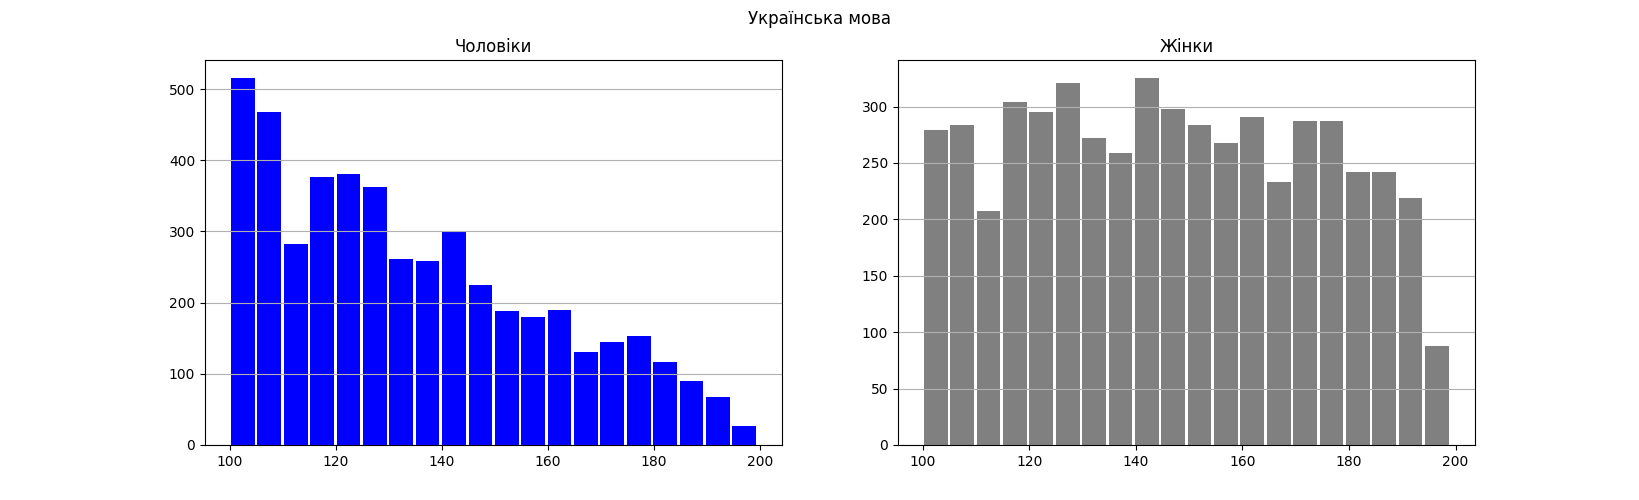
\includegraphics[trim=4cm 0cm 4cm 1cm, clip, width=1\linewidth]{UKR figures/UKR_10000.png}}
    \caption{Результати з української мови}
    \label{fig:UKR initial data}
\end{figure}

На малюнку наведено розподіл балів чоловіків та жінок: неозброєним оком бачимо наявну відмінність отриманих 
оцінок в залежності від статі. З'ясуємо, чи ця відмінність є статистично значущою.

\subsection*{Перевірка гіпотези однорідності даних}
\addcontentsline{toc}{subsection}{Перевірка гіпотези однорідності даних}

Нехай маємо дві незалежні вибірки $\left\{ X_i \right\}$ та $\left\{ Y_j \right\}$ однаково розподілених 
випадкових величин, розподіли $F_x$ й $F_y$ яких нам невідомі:
\begin{align*}
    &X_1 \ldots X_n\sim F_x && \text{результати чоловіків} \\
    &Y_1 \ldots Y_m\sim F_y && \text{результати жінок}
\end{align*}

Перевіримо гіпотезу про однорідність статистичного матеріалу, тобто гіпотезу, що ймовірності 
спостереження умовно високих, помірних та низьких балів в обох вибірках є однаковими. Таким чином 
матимемо $k=2$ вибірок, в яких елементи приймають $s=3$ різних значень. Для формалізації задачі 
введемо позначення:
\[ p_{ij}=\left\{
    \parbox[c]{13cm}{
    оцінка з чоловічо$\text{ї}_{(i=1)}$ чи жіночо$\text{ї}_{(i=2)}$ вибірки належить множині 
    високи$\text{х}_{(j=1)}$, помірни$\text{х}_{(j=2)}$ чи низьки$\text{х}_{(j=3)}$ балів
    } \right\} \]

Категорізація на множини оцінок того чи іншого рівня базувалася на прохідних балах на 
різні факультети КПІ у 2019 році (із переліком прохідних балів можна ознайомитися за 
\href{https://kpi.ua/2019-score}{посиланням}). 

\newpage
При цьому <<високі>> оцінки обиралися із міркувань, що вступнику із таким балом доступно для 
вступу на бюджет більше ніж $65\%$ усіх факультетів, натомість абітурієнту із <<низькими>> 
оцінками рівень доступності значно нижчий -- лише $30\%$. До прикладу: 
\begin{align*}
    &A_1=\{ \text{оцінки, вищі за 178 балів} \} \\
    &A_2=\{ \text{оцінки між 144 та 178 балами} \} \\
    &A_3=\{ \text{оцінки, нижчі за 144 бали} \}
\end{align*}

Остаточно гіпотеза перевірки однорідності спосережуваних даних формулюватиметься так:
\begin{align}
    &\text{нульова гіпотеза} &&H_0: p_{11}=p_{21},\ p_{12}=p_{22},\ p_{13}=p_{23} \label{formula: hypothesis} \\
    &\text{проти альтернативи} && H_1: \exists i,j\quad p_{1,j}\neq p_{2,j} \nonumber
\end{align}

А тоді критерієм перевірки гіпотези слугуватиме правило
\begin{equation}
    \delta(x_1\ldots x_n,\ y_1\ldots y_m)=
    \begin{cases}
    H_1, & \rho\geqslant\chi^2_{1-\alpha;\ (k-1)(s-1)} \\
    H_0, & \rho<\chi^2_{1-\alpha;\ (k-1)(s-1)} \\
    \end{cases}\ , \label{formula: criterion}
\end{equation}

де статистика критерію $\rho$ обчислюється так:
\begin{equation}
    \rho\equiv \rho(x_1\ldots x_n,\ y_1\ldots y_m)=(n+m)\left( \sum\limits_{i=1}^k \sum\limits_{j=1}^s 
    \frac{\vartheta_{ij}^2}{\vartheta_{i\cdot}\vartheta_{\cdot j}} - 1\right), \label{formula: criterion statistics}
\end{equation}

величина критичної точки $\chi^2_{1-\alpha;\ (k-1)(s-1)}$ є квантилем рівня $(1-\alpha)$ розподілу Ст'юдента 
із $(k-1)(s-1)$ степенями свободи, а також
\begin{align*}
    &\vartheta_{1j}=\sum\limits_{i=1}^{n}\mathds{1}(X_i\in A_j) 
        && \parbox[c]{9.3cm}{частота потрапляння елементів вибірки \\ результатів чоловіків в одну із $j$ категорій} \\
    &\vartheta_{2j}=\sum\limits_{i=1}^{m}\mathds{1}(Y_i\in A_j) 
        && \parbox[c]{9cm}{частота потрапляння елементів вибірки \\ результатів жінок в одну із $j$ категорій} \\
    &\vartheta_{i\cdot}=\sum\limits_{j=1}^{s}\vartheta_{ij},\ \vartheta_{\cdot j}=\sum\limits_{i=1}^{k}\vartheta_{ij} 
        && \parbox[c]{9cm}{суми відповідних рядків чи стовпців \\ таблиці спостережуваних даних}
\end{align*}

\newpage
\subsubsection*{Таблиця спостережуваних даних}
\addcontentsline{toc}{subsubsection}{Таблиця спостережуваних даних}

Складемо таблицю за спостережуваними даними навмання обраних $n=500$ та $m=500$ елементів із вибірок 
результатів ЗНО з української мови для чоловіків та жінок:

\begin{table}[H]
    \vspace*{0.8cm}
    \begin{center}
        \begin{tabular}{|c||c|c|c|c|}
            \hline
             & \text{Низькі бали} & \text{Помірні бали} & \text{Високі бали} & \text{Всього} \\
            \hline \hline
            \text{Чоловіки} & 343 & 125 & 32 & 500 \\
            \hline
            \text{Жінки} & 231 & 186 & 83 & 500 \\
            \hline
            \text{Всього} & 574 & 311 & 115 & 1000 \\
            \hline
        \end{tabular}
        \caption{Таблиця спостережуваних значень}
        \label{table: UKR homogeneity data}
    \end{center}
\end{table}

Обчислимо значення статистики критерію:
\begin{equation*}
    \rho = 1000\left( \frac{343^2}{574\cdot 500}+\frac{125^2}{311\cdot 500} + \ldots + 
    \frac{186^2}{311\cdot 500}+\frac{83^2}{115\cdot 500} - 1 \right) = 56.44
\end{equation*}

Водночас на рівні значущості $\alpha=0.01$ значення критичної точки
\begin{equation*} 
    \chi^2_{0.99;\ (2-1)(3-1)}=\chi^2_{0.99;\ 2}=9.21
\end{equation*}

\subsubsection*{Висновок}
\addcontentsline{toc}{subsubsection}{Висновок}

Оскільки значення статистики критерію перевищує значення критичної точки, то згідно критерію 
(\ref{formula: criterion}) гіпотеза про однорідність статистичних даних відхиляється. 
Отже, ймовірності спостереження оцінок різного рівня у вибірках для чоловіків та жінок, 
відповідно, різняться, тобто наявна ситуація неоднакового розполіду балів в залежності від статі.

\subsubsection*{Значення \texttt{p-value}}
\addcontentsline{toc}{subsubsection}{Значення \texttt{p-value}}

Нехай випадкова величина $\tau$ має такий самий розподіл як і статистика критерію й при цьому не залежить 
від неї: $\tau\sim\chi^2(2)$. Тоді величина \texttt{p-value} обчислюється як така ймовірність:
\[ P(\tau>\rho\ |\ H_0)=P(\tau>56.44)=1-P(\tau\leqslant56.44)=1-F_{\tau}(56.44)=0.0001\]

Тож при значенні $\alpha<\texttt{p-value}$ гіпотеза $H_0$ приймалася б.

\subsection*{Побудова довірчого інтервалу для різниці середніх}
\addcontentsline{toc}{subsection}{Побудова довірчого інтервалу для різниці середніх}

Знову маємо дві незалежні вибірки $\left\{ X_i \right\}$ та $\left\{ Y_j \right\}$ 
однаково розподілених випадкових величин, розподіли $F_x$ й $F_y$ яких нам невідомі:
\begin{align*}
    &X_1 \ldots X_n\sim F_x && \text{результати чоловіків} \\
    &Y_1 \ldots Y_m\sim F_y && \text{результати жінок}
\end{align*}

Спробуємо оцінити, в якому інтервалі лежить значення різниці середніх балів для вибірок результатів ЗНО з 
української мови чоловіків та жінок. Якщо у вказаному довірчому інтервалі буде значення 
$\{0\}$, тоді можна стверджувати про відсутність значної відмінності між теоретичними 
математичними сподіваннями цих двох вибірок.

\subsubsection*{Нормалізація даних}
\addcontentsline{toc}{subsubsection}{Нормалізація даних}

Хоча розподіли $F_x$ та $F_y$ оригінальних вибірок $\left\{ X_i \right\}$ й $\left\{ Y_j \right\}$ невідомі, 
через великий обсяг наявних даних можна виокремити $N$ незалежних вибірок виду $X^1\ldots X^N$ й 
$Y^1\ldots Y^N$, які в силу центральної граничної теореми (далі -- ЦГТ) мають нормальний розподіл.

Виконаємо ланцюжок перетворень на прикладі вибірки результатів чоловіків. ЦГТ для великої фіксованої кількості 
$n$ елементів цієї послідовності незалежних однаково розподілених випадкових величин матиме вид:
\begin{equation*}
    \frac{\sum\limits_{i=1}^nX_i-M\sum\limits_{i=1}^nX_i}{\sqrt{D\sum\limits_{i=1}^nX_i}}\approx N(0,1)
\end{equation*}

Використовуючи позначення $\mu_x=MX_i,\ \sigma_x^2=DX_i$, спростимо вираз, скориставшись лінійними 
властивостями дисперсії та математичного сподівання:
\begin{equation*}
    \frac{n\overline{X}-n\mu_x}{\sqrt{n\sigma_x^2}}\approx N(0,1),\ \text{де}\ \overline{X}=\frac{1}{n}\sum\limits_{i=1}^nX_i
\end{equation*}

Залишивши $n$ виключно у знаменнику, виконаємо перетворення:
\begin{equation*}
    \frac{n\overline{X}-n\mu_x}{\sqrt{n\sigma_x^2}}\approx N(0,1)\ \Rightarrow\ 
    \frac{\overline{X}-\mu_x}{\sqrt{\sigma_x^2/n}}\approx N(0,1)\ \Rightarrow\
    \overline{X}\approx N(\mu_x,\tfrac{1}{n}\sigma_x^2)
\end{equation*}

При розгляді такої ж кількості спостережень $n$ аналогічним чином отримуємо знормоване значення 
результатів жінок, де $\mu_y=MY_i,\ \sigma_y^2=DY_i:$
\begin{equation*}
    \overline{Y}\approx N(\mu_y,\tfrac{1}{n}\sigma_y^2)
\end{equation*}

Отже, великий обсяг початкових даних дозволяє розбити оригінальні результати $\left\{ X_i \right\}$ й 
$\left\{ Y_j \right\}$ на значну кількість достатньо великих неперетинних множин, сформованих випадковим чином,
для того, щоб мати змогу застосувати ЦГТ і надалі розглядати набори $\overline{X^1}\ldots \overline{X^N}$ 
та $\overline{Y^1}\ldots \overline{Y^N}$ як незалежні дослідження:
\begin{align}
    &\overline{X^1}\ldots \overline{X^N}\sim N(\mu_x,\tfrac{1}{n}\sigma_x^2) && \text{середні результати чоловіків,} \label{formula: overline{X}} \\
    &\overline{Y^1}\ldots \overline{Y^N}\sim N(\mu_y,\tfrac{1}{n}\sigma_y^2) && \text{середні результати жінок,} \label{formula: overline{Y}}
\end{align}

при цьому
\[ \overline{X^i}=\frac{1}{n}\sum\limits_{j=1}^nX_j,\ \overline{Y^i}=\frac{1}{n}\sum\limits_{j=1}^nY_j,\ i=\overline{1,N} \]

Тож початкові спостережувані результати вдалося перетворити у випадковим чином сформовані незалежні вибірки із 
відомими розподілами. Фактично, проведено процес нормалiзацiї початкових даних. Суть процесу схематично можна 
зобразити на прикладi вибірки $\left\{ X_i \right\}:$
\begin{equation}
    \begin{array}{lr}
        X^1_1 \ldots X^1_n\sim F_x \\
        \hfill{\ldots}\hfill \\
        X^N_1 \ldots X^N_n\sim F_x
    \end{array}
    \xRightarrow[]{\text{ ЦГТ }}
    \begin{array}{lr}
        \sqrt{n}\cdot \dfrac{\overline{X^1}-\mu_x}{\sqrt{\sigma_x^2}}\sim N(0,1) \\
        \hfill{\ldots}\hfill \\
        \sqrt{n}\cdot \dfrac{\overline{X^N}-\mu_x}{\sqrt{\sigma_x^2}}\sim N(0,1)
    \end{array} \label{formula: normalization scheme}
\end{equation}

Повертаючись до отриманих наборів (\ref{formula: overline{X}}) та (\ref{formula: overline{Y}}), переконаємося, 
що новоутворені вибірки справді мають нормальний розподіл. Для цього побудуємо гістограми, які за означенням 
є наближеннями істинних щільностей, а потім візуально оглянемо отримані криві:

\begin{figure}[H]
    \center{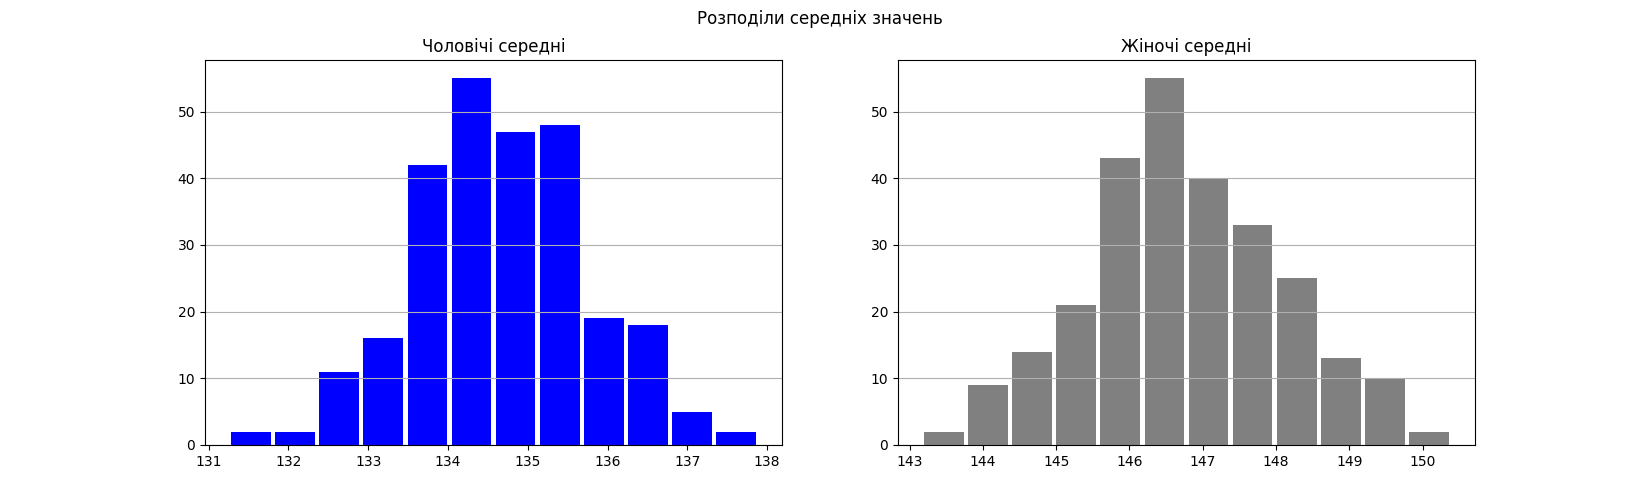
\includegraphics[trim=4cm 0cm 4cm 1cm, clip, width=1\linewidth]{UKR figures/Randomized_means_distribution_m500_N267_v8.png}}
    \caption{Гістограми наборів усереднених результатів ЗНО з української мови}
    \label{fig:UKR means data}
\end{figure}

\newpage
Зауважимо, що криві в обох випадках мають схожі риси (мова про <<висоту>> та <<ширину>> графіків). Тож 
висунемо припущення, що дисперсії цих вибірок однакові: $\sigma_x^2=\sigma_y^2=\sigma^2$. Таким чином 
вирази (\ref{formula: overline{X}}) та (\ref{formula: overline{Y}}) зведуться до такого виду:
\begin{equation}
    \overline{X^1}\ldots \overline{X^N}\sim N(\mu_x,\tfrac{1}{n}\sigma^2),\ 
    \overline{Y^1}\ldots \overline{Y^N}\sim N(\mu_x,\tfrac{1}{n}\sigma^2) \label{formula: X&Y set of means}
\end{equation}

\subsubsection*{Пошук центральної статистики}
\addcontentsline{toc}{subsubsection}{Пошук центральної статистики}
\label{seaching central statistic}

Взявши за основу вибірки (\ref{formula: X&Y set of means}), спробуємо віднайти для параметра 
$\theta=\mu_y-\mu_x$ так звану центральну статистику 
$G(\overline{X^1}\ldots \overline{X^N},\ \overline{Y^1}\ldots \overline{Y^N},\ \theta)\equiv G$, яка має 
задовільняти двом умовам: по-перше, розподіл $f_G(x)$ не залежить від параметра $\theta$, а по-друге, 
функція $G$ неперервна і монотонна за $\theta$.

Перш за все, виходячи з властивостей нормального розподiлу
\begin{equation*} 
    \overline{X}\equiv \tfrac{\overline{X^1}+\ldots +\overline{X^N}}{N} \sim N(\mu_x,\tfrac{1}{Nn}\sigma^2),\ 
    \overline{Y}\equiv \tfrac{\overline{Y^1}+\ldots +\overline{Y^N}}{N} \sim N(\mu_y,\tfrac{1}{Nn}\sigma^2)
\end{equation*}

А отже, розподіл різниці $\overline{Y}-\overline{X}$ матиме вид
\[ \overline{Y}-\overline{X}\sim N(\mu_y-\mu_x,\ \tfrac{2}{Nn}\sigma^2) \]

Тоді позначимо
\begin{equation}
    \xi \equiv \frac{\overline{Y}-\overline{X}-(\mu_y-\mu_x)}{\sqrt{\tfrac{2}{Nn}\sigma^2}} \sim N(0,1) \label{formula: xi}
\end{equation}

Крім того, зазначимо, що
\begin{equation} 
    \frac{(n-1)\left(S_x^2\right)_i}{\sigma^2} \sim \chi^2(n-1),\ 
    \frac{(n-1)\left(S_y^2\right)_i}{\sigma^2} \sim \chi^2(n-1),\ i=\overline{1,N} \label{formula: deviations}
\end{equation}

де
\begin{align*}
    &\begin{array}{lr}
        \left(S_x^2\right)_i=\frac{1}{n-1}\sum\limits_{j=1}^n(X_j^i-\overline{X^i}) \\
        \left(S_y^2\right)_i=\frac{1}{n-1}\sum\limits_{j=1}^n(Y_j^i-\overline{Y^i})
    \end{array} &&
    \parbox[c]{7cm}{
        вибіркові дисперсії двох наборів вибірок середніх результатів
    }
\end{align*}

А отже, сума випадкових величин (\ref{formula: deviations}) як сума незалежних випадкових величин матиме 
розподіл $\chi^2$ із $N(n-1)+N(n-1)$ степенями свободи:
\begin{equation}
    \eta \equiv \frac{(n-1)}{\sigma^2}\left(\sum\limits_{i=1}^N\left(S_x^2\right)_i + \sum\limits_{i=1}^N\left(S_y^2\right)_i\right)\sim \chi^2\left(2N(n-1)\right) \label{formula: eta}
\end{equation}

Тоді випадкова величина
\begin{equation}
    \zeta \overset{\mathrm{def}}{=} \frac{\xi}{\sqrt{\frac{\eta}{2N(n-1)}}} \sim t\left(2N(n-1)\right) \label{formula: zeta}
\end{equation}

Підставивши вирази (\ref{formula: xi}) й (\ref{formula: eta}) у формулу (\ref{formula: zeta}), отримаємо 
шукану центральну статистику для параметра $\theta=\mu_y-\mu_x:$
\begin{equation}
    G=\frac{(\overline{Y}-\overline{X})-\theta}{\sqrt{\tfrac{2}{Nn}}}\cdot 
    \sqrt{\frac{2N(n-1)}{(n-1)(S_X^2+S_Y^2)}}\sim t\left(2N(n-1)\right),
\end{equation}
де 
$ S_X^2=\sum\limits_{i=1}^N\left(S_x^2\right)_i,\ S_Y^2=\sum\limits_{i=1}^N\left(S_y^2\right)_i, $
а статистика $G$ має розподіл Ст'юдента із відповідною кількістю степенів свободи.

\subsubsection*{Побудова довірчого інтервалу}
\addcontentsline{toc}{subsubsection}{Побудова довірчого інтервалу}

Побудуємо довірчий інтервал рівня довіри $\gamma=0.95:$
\[ \gamma \overset{\mathrm{def}}{=} P(g_1<G<g_2)=\int\limits_{g_1}^{g_2}f_G(x)\ dx  \] 

В силу симетричності розподілу Ст'юдента, найкоротший центральний довірчий інтервал матиме вид:
\begin{equation}
    \gamma = P(g_1<G<g_2)=P(|G|<g) \label{formula: gamma interval}
\end{equation}

На малюнку нижче схематично зображено ідею пошуку довірчого інтервалу та визначення відповідного 
квантиля $g:$ 

\begin{figure}[H]
    \center{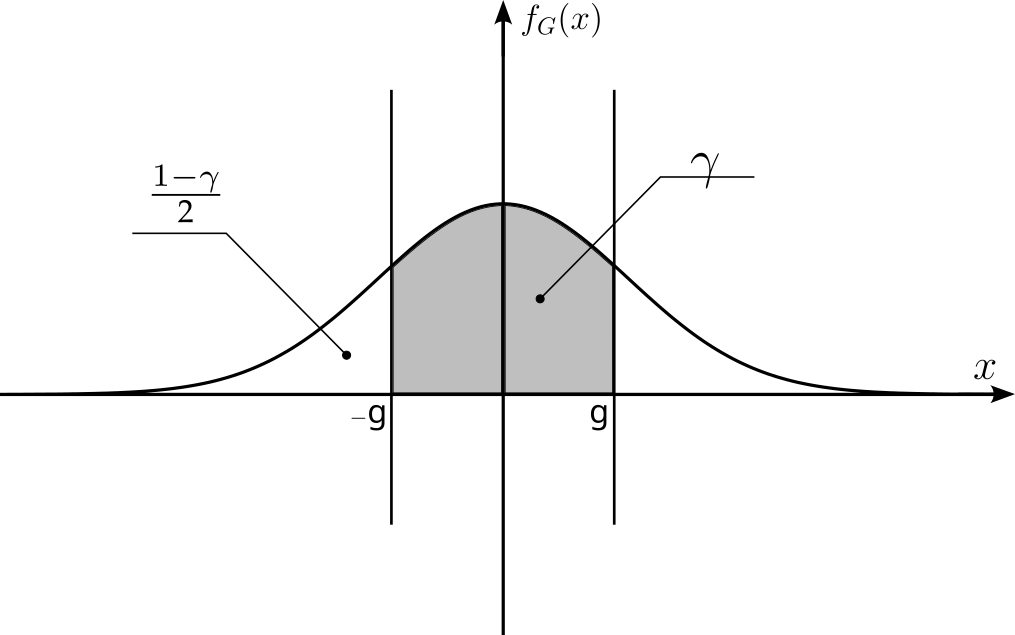
\includegraphics[width=0.9\linewidth]{UKR figures/Interval.png}}
    \caption{Пошук квантиля розподілу Ст'юдента}
    \label{fig:interval}
\end{figure}

Тож враховуючи, що 
$\int\limits_{-\infty}^{\infty}f_G(x)\ dx \overset{\mathrm{def}}{=} 1$, маємо такий ланцюжок міркувань:
\[ \int\limits_{-\infty}^{g}f_G(x)\ dx=\frac{1+\gamma}{2} \
\Rightarrow\ F(g)= \frac{1+\gamma}{2} \
\Rightarrow\ g = t_{\frac{1+\gamma}{2};\ 2N(n-1)} \]

Знайдено квантиль рівня $\frac{1+\gamma}{2}$ розподілу Ст'юдента із $2N(n-1)$ степенями свободи. Підставляючи 
усі отримані результати у формулу (\ref{formula: gamma interval}), отримаємо:
\begin{equation}
    \gamma = P\left(-t_{\tfrac{1+\gamma}{2};\ 2N(n-1)} < \left((\overline{Y}-\overline{X})-\theta\right)\cdot 
    \sqrt{\frac{N^2n}{S_X^2+S_Y^2}} < t_{\tfrac{1+\gamma}{2};\ 2N(n-1)}\right) \label{formula: UKR trusted interval}
\end{equation}

Останнім кроком вкажемо конкретні значення усіх необхідних величин:

\vspace{0.8cm}
\begin{table}[H]
    \begin{center}
        \begin{tabular}{||c|c|c|c|c|c||}
            \hline
            $n$ & $N$ & $g=t_{0.975;\ 2N(n-1)}$ & $S_X^2$ & $S_Y^2$ & $\overline{Y}-\overline{X}$ \\
            \hline \hline
            500 & 267 & 1.96 & 175017.2397 & 200773.7347 & 12.0722 \\
            \hline
        \end{tabular}
        \caption{Значення шуканих параметрів}
        \label{table: UKR interval}
    \end{center}
\end{table}

Підставивши у вираз (\ref{formula: UKR trusted interval}) значення, які наведені у таблиці вище, отримаємо такий довірчий 
інтервал для параметра $\theta=\mu_y-\mu_x$:
\begin{equation*}
    P(11.87 < \theta < 12.27)=0.95
\end{equation*}

\subsubsection*{Висновок}
\addcontentsline{toc}{subsubsection}{Висновок}

Отримано довірчий інтервал рівня довіри $\gamma=0.95$ для величини різниці середніх значень 
оцінок з української мови вибірок результатів чоловіків та жінок: $(11.87,\ 12.27)\ni \mu_y-\mu_x$. Оскільки 
у вказаному проміжку немає нульового значення, гіпотезу про нерозрізнюваність середніх можна відхилити. 

Крім того, візуалізовані дані на Рис. \ref{fig:UKR means data} узгоджуються із отриманим відрізком значень, 
оскільки вершини кривих відрізняються за віссю абсцис приблизно на знай\-дені показники. Можемо стверджувати, 
що при порівнянні результатів чоловіка та жінки оцінка з української мови у жінки буде більшою за оцінку у 
чоловіка на бал у $12.07\pm 0.2$ пункти, при цьому в середньому у п'яти зі ста таких порівнянь вказане 
наближення може бути хибним.